\chapter{Results \textit{\&} Discussion}

\lettrine[
	nindent=0em, findent=0.5em, loversize=-0.12, lines=5
]{\initfamily{T}}{\bfseries\color{Blue}he proposed framework} is tested on the
\gls{uo} database, for predicting \ch{CO2} uptake in \glspl{mof}, the
gas\index{Gas} that mainly ``triggered'' the development of energy-based
descriptors\index{Energy-based descriptors}. In order to evaluate the
transferability of the approach, a different host-guest system is also examined.
We apply the suggested approach in the database created by
\textcite{Mercado_2018}, for predicting \ch{CH4} uptake in \glspl{cof}. In both
cases, the resulting \gls{ml} models are compared with conventional ones, built
upon geometric descriptors\index{Geometric descriptors}. In the rest of this
chapter, results from these comparisons are presented, followed by discussion
for improvements of the proposed framework. Before delving into the results, we
first take a look at RetNet\index{RetNet}, the 3D \gls{cnn} under the hood, that
takes as input a voxelized \gls{pes}\index{Voxelized PES} and outputs a
prediction for a gas adsorption\index{Gas adsorption} property, hereon gas
uptake.

\section{Visualizing RetNet}

Figure \ref{fig:retnet} illustrates the processing a voxelized PES undergoes, as
it is passing through RetNet. For the purpose of this visualization, we use the
model trained on the \glspl{mof} dataset with the largest training set size (see
Section \ref{sec:datasets}). Moreover, for the ease of visualization, only some
feature maps of RetNet are visualized. Please note, that each feature
map\index{Feature map} of a given layer, combines all the feature maps of the
precedent layer. The only exception are the pooling layers\index{Pooling layer},
which just downsample\index{Downsample} the feature maps from the previous
layers.

For example, each feature map of the \conv{2} layer takes into account all
the twelve feature maps of \conv{1} layer. In contrast, the feature maps of the
\pool{1} layer, are just downsampled versions of the corresponding feature maps
in \conv{2} layer. Although feature maps of \glspl{cnn} are not meant to be
interpreted by humans---especially the ones found deeper in the network---it is
worth noticing that early Conv layers\index{Conv layer} (i.e. \conv{1} and
\conv{2}) emphasize the texture of the structure. For instance, the third
feature map of \conv{1} layer delineates the skeleton of the framework.

Moving towards the output layer, the alternation of MaxPool and Conv layers
continues until the Flatten layer\index{Flatten layer}, which just flattens out
and concatenates\footnote{Given $m$ feature maps of size $n \times n \times n$,
a Flatten layer converts them into a vector of size $mn^3$.} all feature maps
from \conv{2} layer into a single vector of size \num{3240}. This vector is then
processed by a \gls{fcnn}---i.e. the stack of Dense\index{Dense layer} and
Output layers---to give the final prediction. Since the Output
layer\index{Output layer} is really nothing more than a linear
layer\index{Linear layer}, all that RetNet does is the following:

\begin{equation}
	\label{eq:retnet}
	\underbrace{\overbrace{\vcx}^\text{PES}}_\text{input}
	\quad \longrightarrow \quad
	\underbrace{
		\overbrace{\phi(\vcx;\vcth)}
		^\text{fingerprint}
	}_\text{feature extraction}
	\quad \longrightarrow \quad
	\underbrace{
		\overbrace{\vc{\beta}^\top\phi(\vcx;\vcth) + \beta_0}
		^\text{gas uptake}
	}_\text{output}
\end{equation}

\begin{figure}
	\centering
	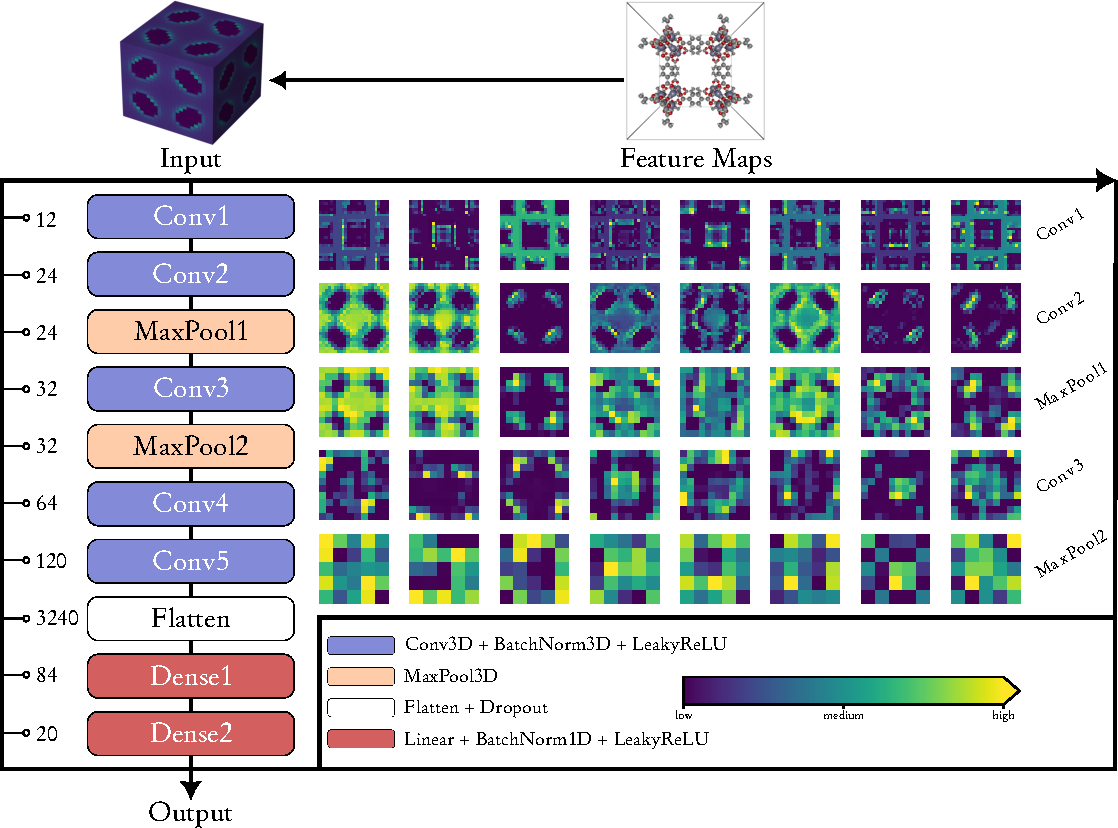
\includegraphics[width=\textwidth]{fig/forward_pass.pdf}
	\caption[RetNet architecture.]{Forward pass\index{Forward pass} of
	IRMOF-1\index{IRMOF-1} through RetNet\index{RetNet}. For the sake of
	visualization, only slices (feature maps\index{Feature map} are 3D matrices)
	of eight feature maps from the first five layers are visualized. For
	\conv{1} layer, the fifth slice is presented, while for the remaining
	layers, the first slice is presented. The IRMOF-1 structure was visualized
	with the iRASPA software \parencite{Dubbeldam2018}.}
	\label{fig:retnet}
\end{figure}

Equation \ref{eq:retnet} says that RetNet, \emph{starting from the PES,
extracts a fingerprint\index{Energetic fingerprint}---that is, a high level
representation\index{High level representation} of the \gls{pes}---and then
predicts the gas uptake by using a linear model on top of this fingerprint}. All
intermediate layers between Input\index{Input layer} and Output layer
participate in this feature extraction step, with the Dense\num{2} layer
determining the size of the fingerprint, which is a vector of size \num{20},
i.e. $\phi(\vcx) \in \mathbb{R}^{20}$ (see Figure \ref{fig:fingerprints}). The
fact that \emph{this fingerprint extraction\index{Fingerprint extraction} step
is learnable}---the parameters $\vcth$ of $\phi$ are learned during the training
phase\index{Training phase}---\emph{is what fundamentally distinguishes the
proposed approach from methods that use hand-crafted
fingerprints\index{Hand-crafted fingerprints}} (see Section
\ref{sec:literature}). \emph{In these methods the fingerprint or
extraction\index{Feature extraction} step is fixed}, and based on some
heuristic, such as energy histograms \parencite{bucior} or average interactions
\parencite{generic}. \emph{Hereon, feature extraction from the \gls{pes} is no
longer fixed, but is an essential part of the training phase}.

\begin{figure}
	\centering
	\begin{subfigure}[b]{0.49\textwidth}
		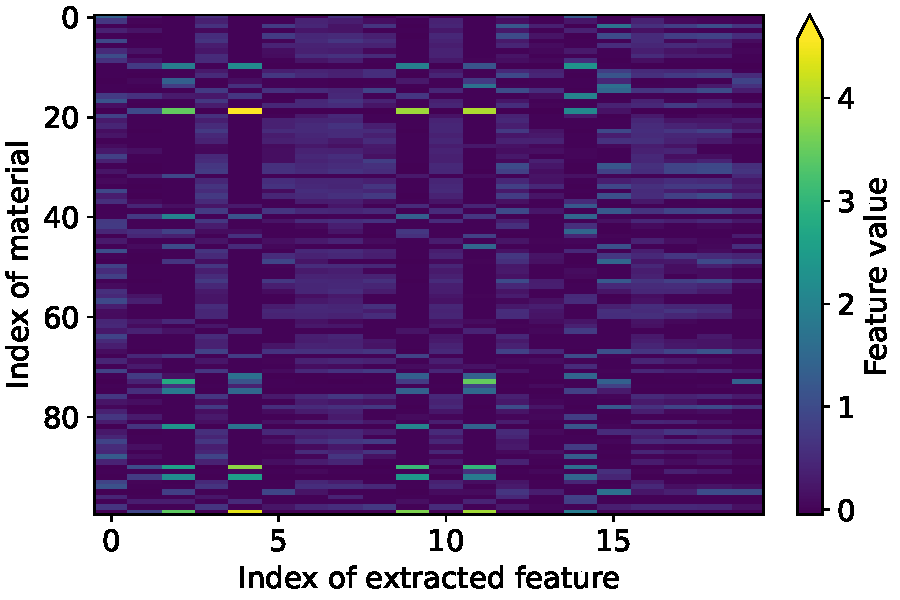
\includegraphics[width=\textwidth]{fig/extracted_features_mofs.pdf}
		\caption{Fingerprints extracted from the \glspl{mof} dataset.}
	\end{subfigure}
	\begin{subfigure}[b]{0.49\textwidth}
		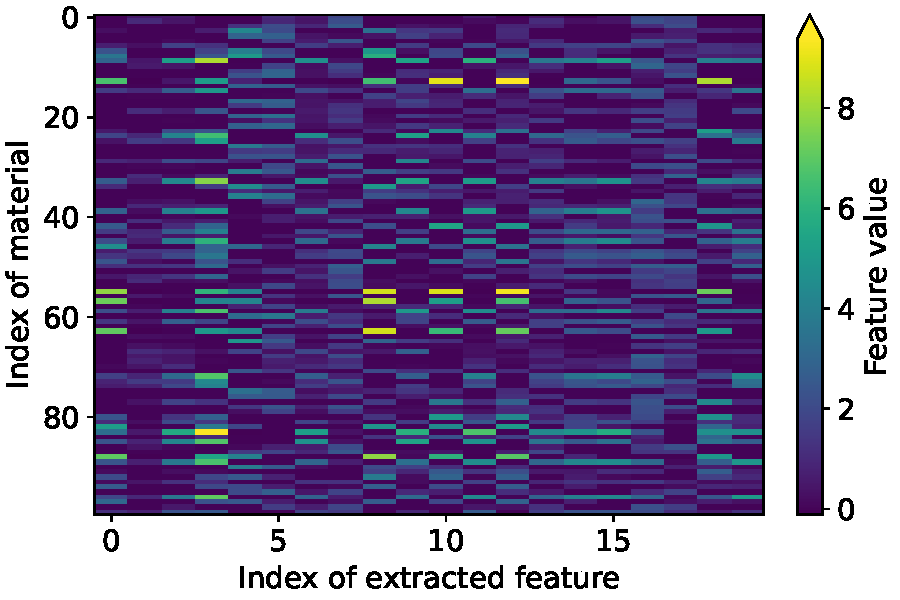
\includegraphics[width=\textwidth]{fig/extracted_features_cofs.pdf}
		\caption{Fingerprints extracted from the \glspl{cof} dataset.}
	\end{subfigure}
	\caption[Fingerprints extracted from RetNet.]{Output of the last LeakyReLU
	layer of RetNet trained on \glspl{mof} (left) and \glspl{cof} (right)
	datasets, with the corresponding maximum training set size. The fingerprints
	of the first \num{100} materials in the training set are depicted.}
	\label{fig:fingerprints}
\end{figure}

\section{Learning Curves}

\begin{figure}
	\centering
	\begin{subfigure}[b]{0.49\textwidth}
		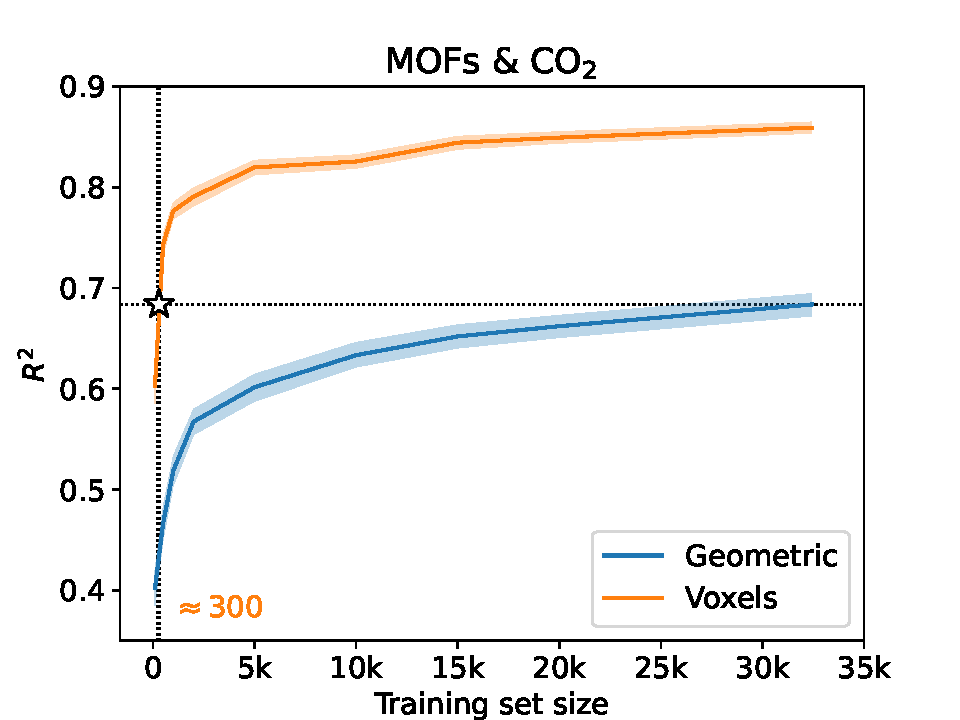
\includegraphics[width=\textwidth]{fig/learning_curves_mofs.pdf}
		\caption{Learning curves for \glspl{mof} \textit{\&} \ch{CO2}.}
		\label{fig:learning_curves_mofs}
	\end{subfigure}
	\begin{subfigure}[b]{0.49\textwidth}
		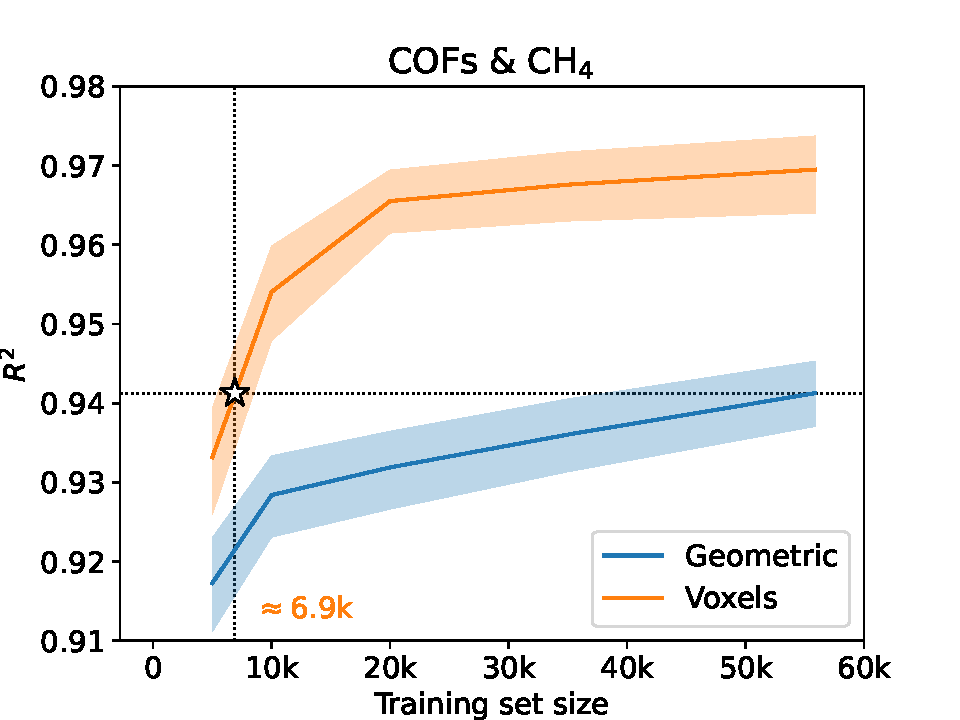
\includegraphics[width=\textwidth]{fig/learning_curves_cofs.pdf}
		\caption{Learning curves for \glspl{cof} \textit{\&} \ch{CH4}.}
		\label{fig:learning_curves_cofs}
	\end{subfigure}
	\caption[Learning curves.]{Performance ($R^2$ score) on test set as function
	of the training set size for conventional and \gls{cnn} models. Shaded areas
	correspond to the \SI{95}{\percent} \gls{ci}\index{Confidence interval}. The
	$x$-coordinate of the white star denotes the trainig set size where the
	\gls{cnn} model reaches the performance of the conventional one, the
	$y$-coordinate. ``Geometric'' stands for geometric descriptors, while
	``Voxels'' stands for energy voxels.}
	\label{fig:learning_curves}
\end{figure}

For the performance boost, please see Section \ref{subsec:data_augmentation}

\section{Discussion}
